\documentclass{extbook}[14pt]
\usepackage{multicol, enumerate, enumitem, hyperref, color, soul, setspace, parskip, fancyhdr, amssymb, amsthm, amsmath, bbm, latexsym, units, mathtools}
\everymath{\displaystyle}
\usepackage[headsep=0.5cm,headheight=0cm, left=1 in,right= 1 in,top= 1 in,bottom= 1 in]{geometry}
\usepackage{dashrule}  % Package to use the command below to create lines between items
\newcommand{\litem}[1]{\item #1

\rule{\textwidth}{0.4pt}}
\pagestyle{fancy}
\lhead{}
\chead{Answer Key for Progress Quiz 4 Version B}
\rhead{}
\lfoot{9187-5854}
\cfoot{}
\rfoot{Spring 2021}
\begin{document}
\textbf{This key should allow you to understand why you choose the option you did (beyond just getting a question right or wrong). \href{https://xronos.clas.ufl.edu/mac1105spring2020/courseDescriptionAndMisc/Exams/LearningFromResults}{More instructions on how to use this key can be found here}.}

\textbf{If you have a suggestion to make the keys better, \href{https://forms.gle/CZkbZmPbC9XALEE88}{please fill out the short survey here}.}

\textit{Note: This key is auto-generated and may contain issues and/or errors. The keys are reviewed after each exam to ensure grading is done accurately. If there are issues (like duplicate options), they are noted in the offline gradebook. The keys are a work-in-progress to give students as many resources to improve as possible.}

\rule{\textwidth}{0.4pt}

\begin{enumerate}\litem{
Which of the following equations \textit{could} be of the graph presented below?

\begin{center}
    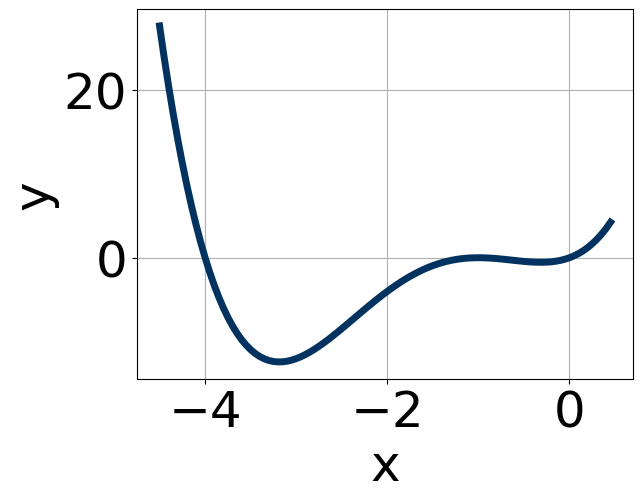
\includegraphics[width=0.5\textwidth]{../Figures/polyGraphToFunctionCopyB.png}
\end{center}


The solution is \( 19x^{5} (x + 1)^{10} (x + 4)^{9} \), which is option A.\begin{enumerate}[label=\Alph*.]
\item \( 19x^{5} (x + 1)^{10} (x + 4)^{9} \)

* This is the correct option.
\item \( -12x^{11} (x + 1)^{4} (x + 4)^{11} \)

This corresponds to the leading coefficient being the opposite value than it should be.
\item \( 13x^{5} (x + 1)^{6} (x + 4)^{4} \)

The factor $(x + 4)$ should have an odd power.
\item \( 5x^{7} (x + 1)^{11} (x + 4)^{4} \)

The factor $-1$ should have an even power and the factor $-4$ should have an odd power.
\item \( -2x^{8} (x + 1)^{10} (x + 4)^{11} \)

The factor $x$ should have an odd power and the leading coefficient should be the opposite sign.
\end{enumerate}

\textbf{General Comment:} General Comments: Draw the x-axis to determine which zeros are touching (and so have even multiplicity) or cross (and have odd multiplicity).
}
\litem{
Describe the end behavior of the polynomial below.
\[ f(x) = -9(x + 4)^{5}(x - 4)^{6}(x + 3)^{2}(x - 3)^{3} \]The solution is the graph below, which is option B.
\begin{center}
    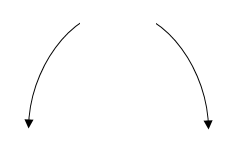
\includegraphics[width=0.3\textwidth]{../Figures/polyEndBehaviorCopyBB.png}
\end{center}\begin{enumerate}[label=\Alph*.]
\begin{multicols}{2}
\item 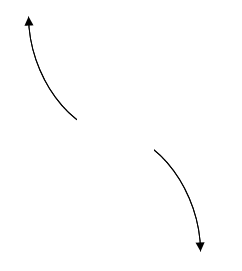
\includegraphics[width = 0.3\textwidth]{../Figures/polyEndBehaviorCopyAB.png}
\item 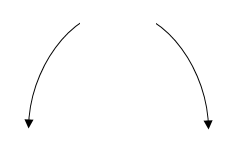
\includegraphics[width = 0.3\textwidth]{../Figures/polyEndBehaviorCopyBB.png}
\item 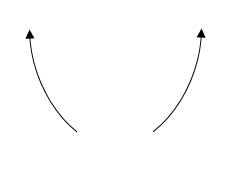
\includegraphics[width = 0.3\textwidth]{../Figures/polyEndBehaviorCopyCB.png}
\item 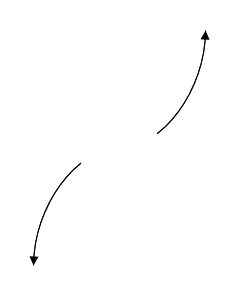
\includegraphics[width = 0.3\textwidth]{../Figures/polyEndBehaviorCopyDB.png}
\end{multicols}\item None of the above.\end{enumerate}
\textbf{General Comment:} Remember that end behavior is determined by the leading coefficient AND whether the \textbf{sum} of the multiplicities is positive or negative.
}
\litem{
Construct the lowest-degree polynomial given the zeros below. Then, choose the intervals that contain the coefficients of the polynomial in the form $ax^3+bx^2+cx+d$.
\[ \frac{-4}{3}, -3, \text{ and } \frac{-6}{5} \]The solution is \( 15x^{3} +83 x^{2} +138 x + 72 \), which is option C.\begin{enumerate}[label=\Alph*.]
\item \( a \in [9, 22], b \in [42, 48], c \in [-30, -28], \text{ and } d \in [-76, -66] \)

$15x^{3} +43 x^{2} -30 x -72$, which corresponds to multiplying out $(3x -4)(x + 3)(5x + 6)$.
\item \( a \in [9, 22], b \in [81, 91], c \in [136, 139], \text{ and } d \in [-76, -66] \)

$15x^{3} +83 x^{2} +138 x -72$, which corresponds to multiplying everything correctly except the constant term.
\item \( a \in [9, 22], b \in [81, 91], c \in [136, 139], \text{ and } d \in [71, 75] \)

* $15x^{3} +83 x^{2} +138 x + 72$, which is the correct option.
\item \( a \in [9, 22], b \in [-85, -80], c \in [136, 139], \text{ and } d \in [-76, -66] \)

$15x^{3} -83 x^{2} +138 x -72$, which corresponds to multiplying out $(3x -4)(x -3)(5x -6)$.
\item \( a \in [9, 22], b \in [-51, -46], c \in [-18, -13], \text{ and } d \in [71, 75] \)

$15x^{3} -47 x^{2} -18 x + 72$, which corresponds to multiplying out $(3x -4)(x -3)(5x + 6)$.
\end{enumerate}

\textbf{General Comment:} To construct the lowest-degree polynomial, you want to multiply out $(3x + 4)(x + 3)(5x + 6)$
}
\litem{
Describe the zero behavior of the zero $x = -2$ of the polynomial below.
\[ f(x) = 5(x - 2)^{9}(x + 2)^{14}(x + 6)^{2}(x - 6)^{3} \]The solution is the graph below, which is option C.
\begin{center}
    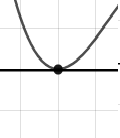
\includegraphics[width=0.3\textwidth]{../Figures/polyZeroBehaviorCB.png}
\end{center}\begin{enumerate}[label=\Alph*.]
\begin{multicols}{2}
\item 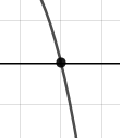
\includegraphics[width = 0.3\textwidth]{../Figures/polyZeroBehaviorAB.png}
\item 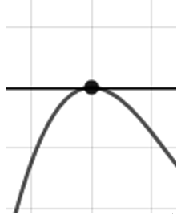
\includegraphics[width = 0.3\textwidth]{../Figures/polyZeroBehaviorBB.png}
\item 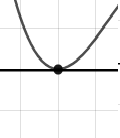
\includegraphics[width = 0.3\textwidth]{../Figures/polyZeroBehaviorCB.png}
\item 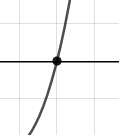
\includegraphics[width = 0.3\textwidth]{../Figures/polyZeroBehaviorDB.png}
\end{multicols}\item None of the above.\end{enumerate}
\textbf{General Comment:} You will need to sketch the entire graph, then zoom in on the zero the question asks about.
}
\litem{
Describe the end behavior of the polynomial below.
\[ f(x) = -6(x - 6)^{5}(x + 6)^{6}(x - 8)^{2}(x + 8)^{3} \]The solution is the graph below, which is option B.
\begin{center}
    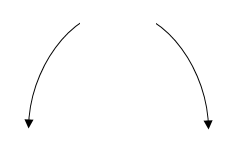
\includegraphics[width=0.3\textwidth]{../Figures/polyEndBehaviorBB.png}
\end{center}\begin{enumerate}[label=\Alph*.]
\begin{multicols}{2}
\item 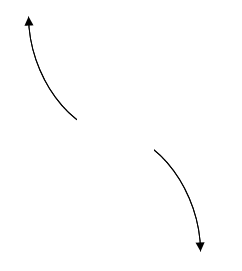
\includegraphics[width = 0.3\textwidth]{../Figures/polyEndBehaviorAB.png}
\item 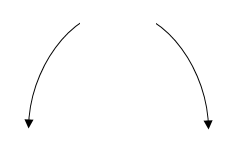
\includegraphics[width = 0.3\textwidth]{../Figures/polyEndBehaviorBB.png}
\item 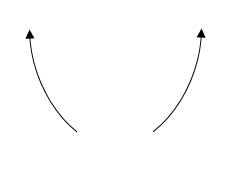
\includegraphics[width = 0.3\textwidth]{../Figures/polyEndBehaviorCB.png}
\item 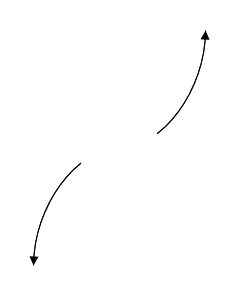
\includegraphics[width = 0.3\textwidth]{../Figures/polyEndBehaviorDB.png}
\end{multicols}\item None of the above.\end{enumerate}
\textbf{General Comment:} Remember that end behavior is determined by the leading coefficient AND whether the \textbf{sum} of the multiplicities is positive or negative.
}
\litem{
Construct the lowest-degree polynomial given the zeros below. Then, choose the intervals that contain the coefficients of the polynomial in the form $x^3+bx^2+cx+d$.
\[ -3 - 2 i \text{ and } -1 \]The solution is \( x^{3} +7 x^{2} +19 x + 13 \), which is option C.\begin{enumerate}[label=\Alph*.]
\item \( b \in [-0.9, 1.1], c \in [3.8, 5.6], \text{ and } d \in [2.51, 3.71] \)

$x^{3} + x^{2} +4 x + 3$, which corresponds to multiplying out $(x + 3)(x + 1)$.
\item \( b \in [-0.9, 1.1], c \in [2.8, 3.5], \text{ and } d \in [1.06, 2.89] \)

$x^{3} + x^{2} +3 x + 2$, which corresponds to multiplying out $(x + 2)(x + 1)$.
\item \( b \in [5.9, 10.8], c \in [17.6, 19.4], \text{ and } d \in [12.15, 13.95] \)

* $x^{3} +7 x^{2} +19 x + 13$, which is the correct option.
\item \( b \in [-8, -3.3], c \in [17.6, 19.4], \text{ and } d \in [-13.5, -12.06] \)

$x^{3} -7 x^{2} +19 x -13$, which corresponds to multiplying out $(x-(-3 - 2 i))(x-(-3 + 2 i))(x -1)$.
\item \( \text{None of the above.} \)

This corresponds to making an unanticipated error or not understanding how to use nonreal complex numbers to create the lowest-degree polynomial. If you chose this and are not sure what you did wrong, please contact the coordinator for help.
\end{enumerate}

\textbf{General Comment:} Remember that the conjugate of $a+bi$ is $a-bi$. Since these zeros always come in pairs, we need to multiply out $(x-(-3 - 2 i))(x-(-3 + 2 i))(x-(-1))$.
}
\litem{
Which of the following equations \textit{could} be of the graph presented below?

\begin{center}
    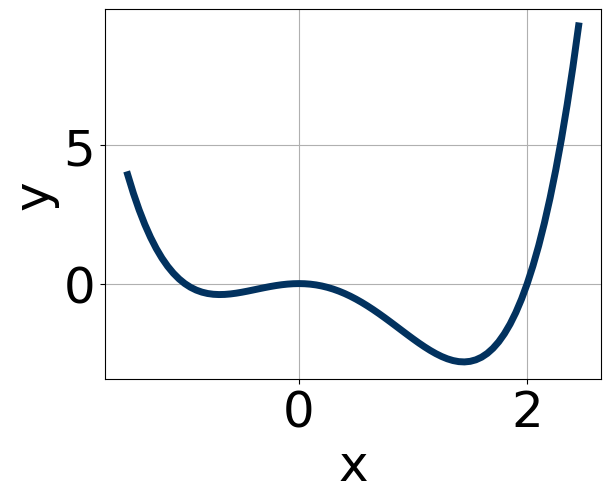
\includegraphics[width=0.5\textwidth]{../Figures/polyGraphToFunctionB.png}
\end{center}


The solution is \( -17x^{9} (x + 4)^{7} (x - 2)^{11} \), which is option E.\begin{enumerate}[label=\Alph*.]
\item \( -12x^{4} (x + 4)^{10} (x - 2)^{11} \)

The factors $0$ and $-4$ have have been odd power.
\item \( 15x^{8} (x + 4)^{11} (x - 2)^{11} \)

The factor $x$ should have an odd power and the leading coefficient should be the opposite sign.
\item \( -15x^{6} (x + 4)^{11} (x - 2)^{7} \)

The factor $0$ should have been an odd power.
\item \( 17x^{11} (x + 4)^{7} (x - 2)^{7} \)

This corresponds to the leading coefficient being the opposite value than it should be.
\item \( -17x^{9} (x + 4)^{7} (x - 2)^{11} \)

* This is the correct option.
\end{enumerate}

\textbf{General Comment:} General Comments: Draw the x-axis to determine which zeros are touching (and so have even multiplicity) or cross (and have odd multiplicity).
}
\litem{
Construct the lowest-degree polynomial given the zeros below. Then, choose the intervals that contain the coefficients of the polynomial in the form $x^3+bx^2+cx+d$.
\[ 5 + 2 i \text{ and } -3 \]The solution is \( x^{3} -7 x^{2} -x + 87 \), which is option B.\begin{enumerate}[label=\Alph*.]
\item \( b \in [5, 11], c \in [-1.05, -0.7], \text{ and } d \in [-96, -81] \)

$x^{3} +7 x^{2} -x -87$, which corresponds to multiplying out $(x-(5 + 2 i))(x-(5 - 2 i))(x -3)$.
\item \( b \in [-13, -2], c \in [-1.05, -0.7], \text{ and } d \in [87, 93] \)

* $x^{3} -7 x^{2} -x + 87$, which is the correct option.
\item \( b \in [-2, 5], c \in [-2.32, -1.02], \text{ and } d \in [-17, -12] \)

$x^{3} + x^{2} -2 x -15$, which corresponds to multiplying out $(x -5)(x + 3)$.
\item \( b \in [-2, 5], c \in [0.87, 1.64], \text{ and } d \in [-6, -1] \)

$x^{3} + x^{2} +x -6$, which corresponds to multiplying out $(x -2)(x + 3)$.
\item \( \text{None of the above.} \)

This corresponds to making an unanticipated error or not understanding how to use nonreal complex numbers to create the lowest-degree polynomial. If you chose this and are not sure what you did wrong, please contact the coordinator for help.
\end{enumerate}

\textbf{General Comment:} Remember that the conjugate of $a+bi$ is $a-bi$. Since these zeros always come in pairs, we need to multiply out $(x-(5 + 2 i))(x-(5 - 2 i))(x-(-3))$.
}
\litem{
Describe the zero behavior of the zero $x = 3$ of the polynomial below.
\[ f(x) = -8(x + 3)^{8}(x - 3)^{13}(x - 7)^{3}(x + 7)^{7} \]The solution is the graph below, which is option D.
\begin{center}
    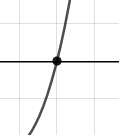
\includegraphics[width=0.3\textwidth]{../Figures/polyZeroBehaviorCopyDB.png}
\end{center}\begin{enumerate}[label=\Alph*.]
\begin{multicols}{2}
\item 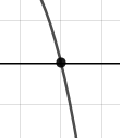
\includegraphics[width = 0.3\textwidth]{../Figures/polyZeroBehaviorCopyAB.png}
\item 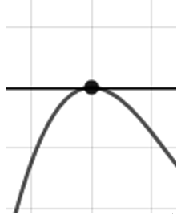
\includegraphics[width = 0.3\textwidth]{../Figures/polyZeroBehaviorCopyBB.png}
\item 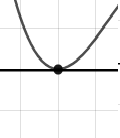
\includegraphics[width = 0.3\textwidth]{../Figures/polyZeroBehaviorCopyCB.png}
\item 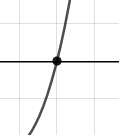
\includegraphics[width = 0.3\textwidth]{../Figures/polyZeroBehaviorCopyDB.png}
\end{multicols}\item None of the above.\end{enumerate}
\textbf{General Comment:} You will need to sketch the entire graph, then zoom in on the zero the question asks about.
}
\litem{
Construct the lowest-degree polynomial given the zeros below. Then, choose the intervals that contain the coefficients of the polynomial in the form $ax^3+bx^2+cx+d$.
\[ \frac{6}{5}, \frac{2}{3}, \text{ and } \frac{-1}{5} \]The solution is \( 75x^{3} -125 x^{2} +32 x + 12 \), which is option D.\begin{enumerate}[label=\Alph*.]
\item \( a \in [70, 76], b \in [-125, -119], c \in [32, 39], \text{ and } d \in [-13, 1] \)

$75x^{3} -125 x^{2} +32 x -12$, which corresponds to multiplying everything correctly except the constant term.
\item \( a \in [70, 76], b \in [125, 126], c \in [32, 39], \text{ and } d \in [-13, 1] \)

$75x^{3} +125 x^{2} +32 x -12$, which corresponds to multiplying out $(5x + 6)(3x + 2)(5x -1)$.
\item \( a \in [70, 76], b \in [53, 60], c \in [-59, -48], \text{ and } d \in [-13, 1] \)

$75x^{3} +55 x^{2} -52 x -12$, which corresponds to multiplying out $(5x + 6)(3x -2)(5x + 1)$.
\item \( a \in [70, 76], b \in [-125, -119], c \in [32, 39], \text{ and } d \in [11, 16] \)

* $75x^{3} -125 x^{2} +32 x + 12$, which is the correct option.
\item \( a \in [70, 76], b \in [154, 164], c \in [88, 90], \text{ and } d \in [11, 16] \)

$75x^{3} +155 x^{2} +88 x + 12$, which corresponds to multiplying out $(5x + 6)(3x + 2)(5x + 1)$.
\end{enumerate}

\textbf{General Comment:} To construct the lowest-degree polynomial, you want to multiply out $(5x -6)(3x -2)(5x + 1)$
}
\end{enumerate}

\end{document}